\documentclass[12pt]{article}
	
%______________________PREAMBULO_________________________

%----------------------Paquetes--------------------------
\usepackage{amsmath,amssymb,amsfonts,latexsym,cancel} % Paquetes de símbolos adicionales.
\usepackage[spanish,es-tabla]{babel} % Idioma español
\usepackage[utf8]{inputenc} % Paquete que nos permite usar los acentos y otros símbolos, directamente del teclado.
\usepackage[T1]{fontenc} % Cambia el tipo de letra
\usepackage{times} % Tipo de letra Times New Roman
\usepackage{graphicx} % Paquete para el manejo de gráficos y figuras en el documento.
\usepackage{geometry} % Permite el manejo de los margenes
\usepackage{fancyhdr} % Permite colocar y manejar el encabezado
\usepackage[breaklinks,colorlinks=true,linkcolor=black,citecolor=blue, urlcolor=blue]{hyperref} % Crea hipervinculo entre secciones y el indice
\usepackage{pstricks}
\usepackage{multicol}
%\usepackage{mathpazo} %fuente palatino
%\usepackage{xcolor}
%\usepackage[shortlabels]{enumitem}
%-------------Paquetes para el formato de las citas-------
%\usepackage[hyphens]{url}
%\usepackage{float}
%\usepackage{cite}
%\usepackage{wrapfig}

%-----------------------------ayuda de paquetes--------------------

\spanishdecimal{.}

%------------------------Margenes----------------------------

\newgeometry{bottom = 2.5 cm, top = 2.5 cm, left = 2 cm, right = 2 cm} % Modifica el margen {Abajo, Arriba, Izquierda, Derecha

%----------------------------Interlineado----------------------------------

%\doublespacing
%\onehalfspace
%\singlespace
%\spacing{1.5} % Permite personalisar a gusto
%\setlength{\parskip}{2cm} % Es el espacio entre parrafos

%-----------------------------Sangria---------------------------------------

\setlength{\parindent}{0 cm} % Manipula la sangria

%---------------------Portada------------------

%\title{
%\begin{figure}[h!]
		
%	\centering
%	
\includegraphics[width=\linewidth]{Nom_UAdeC_FCFM.png}  			
			
%\end{figure}
%\huge \textbf{LABORATORIO DE FISICA 3}\\\LARGE TITULO PRACTICA\\}
%\author{ \Large \textbf{Profesor:}\\
%\Large \textbf{Alumno:} Oscar Joel Castro Contreras}
%\date{\today}

%--------------Encabezado y pie de pagina--------------------

\pagestyle{fancy}%Coloca el encabezado en el documento
\lhead[]{Métodos numéricos}%Encabezado izquierda
\rhead[]{Oscar Joel Castro Contreras}%Encabesado derecha
%\chead[]{}%Encabesado central
\renewcommand{\headrulewidth}{0.08 pt}%Coloca linea al pie de pagina

%\lfoot[]{PI}%Pie de pagina izquerdo
%\rfoot[]{PD}%Pie de pagina derecho
\cfoot[]{\thepage}%Pie de pagina central
\renewcommand{\footrulewidth}{0.08 pt}%Coloca linea al pie de pagina

%-----------------------------------------------------------------------------

	\begin{document}
		
		\begin{titlepage}
		
			\centering
			{\bfseries
			\begin{figure}[h!]
				\centering
				
\includegraphics[width=\linewidth]{Nom_UAdeC_FCFM.png} 				
			\end{figure}
			\par}
			\vspace{2cm}
			{\scshape\LARGE Métodos numéricos \par}
			\vspace{3cm}
			{\scshape\Huge \textbf{Método de Müller} \par}
			\vfill
			{\LARGE \textbf{Profesora:} Maria Guadalupe Godina Cubillo \par}
			\vspace{3cm}
			{\LARGE \textbf{Alumno:} Oscar Joel Castro Contreras \par}
			\vfill
			{\Large \today \par}
			\thispagestyle{empty}
			%\thispagestyle{fancy}
			
		\end{titlepage}
	
		\newpage

		\begin{abstract}
			\noindent En este reporte explico un poco de los métodos que existen para encontrar las raíces de cualquier 
			polinomio o función que tenga raíces, y en específico explico, qué es, en que consiste y cuales son las 
			limitaciones del método de Müller para encontrar raíces reales y imaginarias.
		\end{abstract}

		\textbf{Palabras clave:} Raíces imaginarias, Müller, Numero complejo.

		\section*{\centering Introducción}\label{sec:Introducción}
			Los polinomios son uno de los conceptos más importantes en álgebra y son fundamentales en 
			matemáticas y ciencia en general. Determinar las raíces de un polinomio es uno de los problemas 
			más antiguos en matemáticas.\\
			Puesto que las ecuaciones polinomiales aparecen en un amplio rango de áreas de la ciencia, desde 
			química y física básica hasta economía, el problema de determinar raíces de polinomios es, con 
			frecuencia, un paso obligado en la resolución de problemas.\cite{bib:item1}\\
			La razón principal para resolver ecuaciones no lineales por medio de métodos computacionales es 
			que algunas ecuaciones carecen de solución exacta, excepto por unas pocas. Por lo que existen 
			métodos numéricos diseñados para obtener las raíces, aunque cada uno tiene sus propias 
			limitaciones y defectos. Algunos métodos se muestran en la tabla \ref{tab:1}.\cite{bib:item2}\\
			\begin{table}[h!]
				\centering
				\begin{tabular}{|c|c|}
					\hline
					\multicolumn{2}{|c|}{\textbf{Métodos numéricos para obtener raíces}}\\
					\hline
					\textbf{Nombre} & \textbf{Características} \\\hline
					Bisección & Aplicable a funciones no analiticas \\\hline
					Regla falsa & Convergencia lenta en un intervalo grande \\\hline								
					Método de Newton & Rápido, se nesecita calcular derivada \\\hline
					Método de secante & Rápido, no se requiera calcular derivada \\\hline
					Sustitución sucesiva & Puede no converger \\\hline
				\end{tabular}
				\caption{Métodos numéricos para obtener raíces \cite{bib:item2}}
				\label{tab:1}
			\end{table}\\
			En general, no es posible determinar los ceros de una función, es decir, valores $ x^* $ tal que $f(x^*) = 0 $, 
			en un número finito de pasos. Tenemos que usar métodos de aproximación. Los métodos son 
			usualmente iterativos y tienen la forma: Iniciando con una aproximación inicial $ x_0 $ (o un intervalo $ [a,b] $) , 
			se calculan aproximaciones sucesivas $ x_1,x_2,... $ y elegimos $ x_n $ como aproximación de $ x^* $ cuando se cumpla un 
			criterio de parada dado. A los ceros de un polinomio se les conoce también como raíces.\\
			\textbf{El método de Müller:}\\
			El método de Müller se puede usar para encontrar cualquier tipo de raíz, real o compleja, de una 
			función arbitraria. Su aplicación requiere valores iniciales y es una extensión del método de la 
			secante. Se toman tres valores iniciales $ x_0, x_1, x_2 $ y se halla el polinomio $ p(x) $ de 
			segundo grado que pasa por los puntos $ (x_0,f(x_0)), (x_1,f(x_1)),(x_2,f(x_2)) $, y se toma una 
			de las raíces de $ p(x) $, la mas cercana a $ x_2 $, como la siguiente aproximación $ x_3 $. Se 
			repite la operación con los nuevos valores iniciales $ x_1, x_2, x_3 $, y se termina el proceso 
			tan pronto como se satisfaga algún criterio de convergencia.\cite{bib:item3}

		\section*{\centering Metodología}\label{sec:Metodologia}
			El método de Müller parte de tres puntos $ x_0, x_1, x_2 $ aproximados a las raíces del polinomio 
			sin importara si es real o compleja. Con estos 3 puntos creamos una ecuación cuadrática $ p(x) $ 
			que los cruce.\\
			Esta ecuación la obtenemos tomando el polinomio cuadrático $$ p(x) = a(x-x_2)^2 + b(x-x_2) + c $$
			que pasa por $$ (x_0,f(x_0)), (x_1,f(x_1)),(x_2,f(x_2)). $$ Para obtener los componentes $ a, b $ y $ c $
			es apartir de las siguientes condiciones
			\begin{align*}
				f(x_0) &= a(x_0-x_2)^2 + b(x_0-x_2) + c \\
				f(x_1) &= a(x_1-x_2)^2 + b(x_1-x_2) + c \\
				f(x_2) &= a(x_2-x_2)^2 + b(x_2-x_2) + c = c
			\end{align*}
			Podemos ver que ya obtuvimos lo que vale $ c $. De esto tomamos a
			$$ h_0 = x_0-x_2 $$
			$$ h_1 = x_1-x_2 $$
			y podemos decir que
			\begin{align*}
				f(x_0) &= ah_0^2 + bh_0 + c \\
				f(x_0) - c &= ah_0^2 + bh_0 \\\\
				f(x_1) &= ah_1^2 + bh_1 + c\\
				f(x_1) - c &= ah_1^2 + bh_1 
			\end{align*}
			De esto tomamos que
			$$ e_0 = f(x_0)-c $$
			$$ e_1 = f(x_1)-c $$
			Ahora resolvemos el sistema
			\begin{align*}
				e_0 &= ah_0^2 + bh_0 \\
				e_1 &= ah_1^2 + bh_1 
			\end{align*}
			y tomando a $$ w = h_1-h_0^2 - h_1^2-h_0 $$ \\
			llegamos a que
			\begin{align*}
				a &= \frac{e_0h_1 - e_1h_0}{w} \\
				b &= \frac{e_1h_0^2 - h_1^2e_0}{w} \\
			\end{align*}
			Después, de obtener los coeficientes de la ecuación cuadratica hacemos una aproximación nueva 
			a la raíz $ x_3 $ con la ayuda de la formula cuadratica, modifica para reducir el error.
			$$ x_3 = x_2 - \frac{2c}{b\pm\sqrt{b^2-4ac}} $$
			Al final iteramos con uno de los puntos anteriores la nueva aproximación y ahora realizamos el 
			proceso pero con los puntos $ x_1, x_2, x_3 $, esto se repite hasta que se llega a un abuena 
			aproximación de la raíz real o compleja.
		\section*{\centering Resultado}\label{sec:Resultado}
			Si tomamos el polinomio $ x^3-2x^2-1 $ y damos los punto $ x_0 = -1,\,x_1 = 0,\,x_2 = 1 $. Hacemos 
			la evaluación para obtener la raíz con 5 cifras significativas, el programa nos arroja
			\begin{multicols}{2}
				\begin{center}
					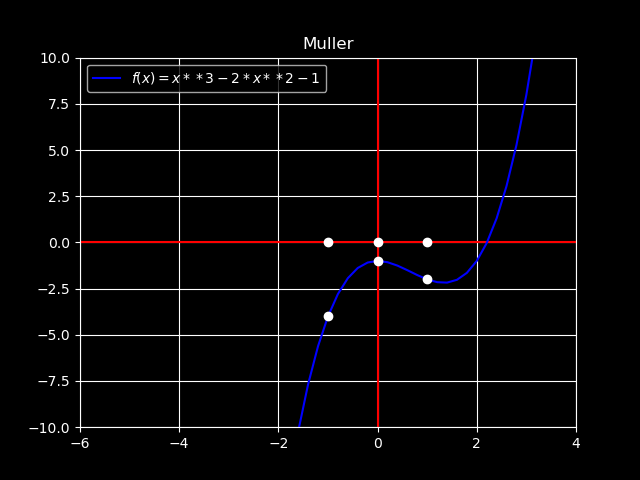
\includegraphics[width=\linewidth]{Grafica 1.png}
					Grafica 1: Valores iniciales dados en la ecuación \columnbreak $ x^3-2x^2-1 $.\\
					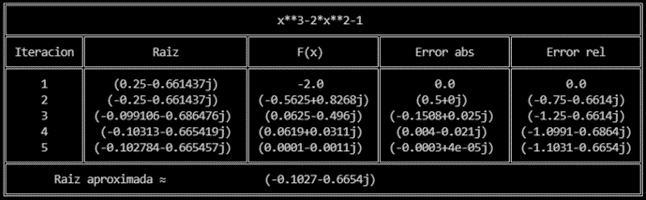
\includegraphics[width=\linewidth]{Tabla 1.png}
					Tabla 2: Iteraciones a la aproximación de la raíz de la función $ x^3-2x^2-1 $.
				\end{center}
			\end{multicols}
			Observamos que la aproximación a una raíz compleja es $ -0.1027 - 0.6654i $, con 5 iteraciones.
		\section*{\centering Observación}\label{sec:Observacion}
			La única limitación que tiene el método es cuando $ w = 0 $, ya que en estos casos no se podría 
			crear la ecuación cuadrática debido a que $ a $ y $ b $ dependen de $ w $. Pero esa sería la única 
			y en muy pocas ocasiones esto ocurre.

		\section*{\centering Conclusión}\label{sec:Conclusion}
			En conclusión, el método de Müller toma 3 puntos cercanos a cualquier raíz real o compleja de 
			cualquier función, de estos puntos crea una ecuación cuadrática que cruce por los puntos y se 
			calcula una aproximación a la raíz de la función con la ayuda de la función cuadrática.\\

		\centering
		\begin{thebibliography}{10}
			\bibitem{bib:item1} de la Vega, H. M. El calculo de raıces de polinomios. Una historia sin fin. Recuperado de
							\href{http://www.matedu.cinvestav.mx/~elcalculoysuensenanza/investigacion/articulosPDF/Madrid.pdf}{Pagina web de \cite{bib:item1}}.
			\bibitem{bib:item2} Nakamura, S. (1998). Metodos Numericos Aplicados Con Software. En Solución de ecuaciones no lineales (Primera ed., pp. 62–63). Prentice Hall.
							\href{https://bibliotecadigital.univalle.edu.co/bitstream/handle/10893/21225/CB%200525927-3487.pdf?sequence=1&isAllowed=y}{Pagina web de \cite{bib:item3}}.
			\bibitem{bib:item3}	Federico, D. S. C., Antonio, N. H. (2014). Métodos Numéricos Aplicados a la Ingeniería. En Método de Müller (Primera ed., pp. 79–85). Grupo Editorial Patria.
		\end{thebibliography}

	\end{document}